\documentclass[12pt, a4]{article}
\usepackage[english]{babel}
\usepackage[utf8x]{inputenc}
\usepackage{fullpage}
\usepackage{listings}
\usepackage{graphicx}
\usepackage{color}

%Syntax highlighting
\definecolor{blue-violet}{rgb}{0.54, 0.17, 0.89}
\definecolor{ao}{rgb}{0.0, 0.5, 0.0}
\definecolor{amaranth}{rgb}{0.9, 0.17, 0.31}
\definecolor{ballblue}{rgb}{0.13, 0.67, 0.8}
\definecolor{onyx}{rgb}{0.06, 0.06, 0.06}


\lstset{
  breaklines=true,                 % automatic line breaking only at whitespace
  captionpos=b,                    % sets the caption-position to bottom
  breakatwhitespace=false,
  keepspaces=true,
  numbers=left,
  numbersep=5pt,
  showspaces=false,
  showstringspaces=false,
  showtabs=false,
  tabsize=4,  
  backgroundcolor=\color{white},   % choose the background color
  commentstyle=\color{ao},    % comment style
  keywordstyle=\color{amaranth},    % keyword style
  stringstyle=\color{blue-violet},    % string literal style
  numberstyle=\tiny\color{ballblue},	   % number style
  basicstyle=\ttfamily\footnotesize\color{onyx} % size of fonts used for the code
}

%Document Header
\title{\textbf{Department of CSE\\SSN College of Engineering}}
\author{\textbf{Vishakan Subramanian - 18 5001 196 - Semester VII}}
\date{22 August 2021}

\begin{document}
\maketitle
\hrule
\section*{\center{UCS 1711 - Mobile Application Development Lab}}
\hrule
\bigskip

%Assignment Details
\subsection*{\center{\textbf{Exercise 4: Android Application Development Using Database}}}
\subsection*{\flushleft{Aim:}}
\begin{flushleft}
To develop an Android application that generates the following using graphical primitives.

In main activity have the following buttons:
Create, Insert, Update, Delete, Retrieve

\begin{enumerate}
\item On clicking Create Button, create a new database to store the following contents. (Use SQLite Database)
\begin{enumerate}
\item Name
\item Gender
\item Employee Code
\item Department
\item Salary
\end{enumerate}

\newpage

\item On Clicking Insert, move to a new view which contains the following details: (Insert new Employee to the database)
\begin{enumerate}
\item Name			(EditText - Validation checking - Alphabet)
\item Gender		(RadioButton)
\item Employee Code	(EditText - Validation checking - Alphanumeric)
\item Department	(Spinner)
\item Salary		(EditText - Validation checking - Numeric)
\item Submit		(Button – On press, Insert the data into database)
\end{enumerate}

\item On clicking Update, move to a new view which contains above details and Update by Employee Code.
\item On clicking Delete, Delete the whole row in the table by Employee Code.
\item On clicking Retrieve, Retrieve an employee by Employee Code. Also retrieve the details of all the employees in a particular department.

\end{enumerate}


\end{flushleft}

%Code
\newpage
\subsection*{\flushleft{Code: Main Activity:}}
\begin{flushleft}
\lstinputlisting[language = Java]{EmployeeManager/app/src/main/java/com/example/employeemanager/MainActivity.java}
\end{flushleft}

%Code
\newpage
\subsection*{\flushleft{Code: Insert Activity:}}
\begin{flushleft}
\lstinputlisting[language = Java]{EmployeeManager/app/src/main/java/com/example/employeemanager/InsertActivity.java}
\end{flushleft}

%Code
\newpage
\subsection*{\flushleft{Code: Update Activity:}}
\begin{flushleft}
\lstinputlisting[language = Java]{EmployeeManager/app/src/main/java/com/example/employeemanager/UpdateActivity.java}
\end{flushleft}

%Code
\newpage
\subsection*{\flushleft{Code: Delete Activity:}}
\begin{flushleft}
\lstinputlisting[language = Java]{EmployeeManager/app/src/main/java/com/example/employeemanager/DeleteActivity.java}
\end{flushleft}

%Code
\newpage
\subsection*{\flushleft{Code: Retrieve Activity:}}
\begin{flushleft}
\lstinputlisting[language = Java]{EmployeeManager/app/src/main/java/com/example/employeemanager/RetrieveActivity.java}
\end{flushleft}

%Code
\newpage
\subsection*{\flushleft{Code: Retrieve Many Activity:}}
\begin{flushleft}
\lstinputlisting[language = Java]{EmployeeManager/app/src/main/java/com/example/employeemanager/RetrieveManyActivity.java}
\end{flushleft}

%Code
\newpage
\subsection*{\flushleft{Code: Employee Database Helper:}}
\begin{flushleft}
\lstinputlisting[language = Java]{EmployeeManager/app/src/main/java/com/example/employeemanager/EmployeeDatabaseHelper.java}
\end{flushleft}


%Code
\newpage
\subsection*{\flushleft{Code: Main Activity Layout}}
\begin{flushleft}
\lstinputlisting[language = XML]{EmployeeManager/app/src/main/res/layout/activity_main.xml}
\end{flushleft}

%Code
\newpage
\subsection*{\flushleft{Code: Insert Activity Layout}}
\begin{flushleft}
\lstinputlisting[language = XML]{EmployeeManager/app/src/main/res/layout/activity_insert.xml}
\end{flushleft}

%Code
\newpage
\subsection*{\flushleft{Code: Update Activity Layout}}
\begin{flushleft}
\lstinputlisting[language = XML]{EmployeeManager/app/src/main/res/layout/activity_update.xml}
\end{flushleft}

%Code
\newpage
\subsection*{\flushleft{Code: Delete Activity Layout}}
\begin{flushleft}
\lstinputlisting[language = XML]{EmployeeManager/app/src/main/res/layout/activity_delete.xml}
\end{flushleft}

%Code
\newpage
\subsection*{\flushleft{Code: Retrieve Activity Layout}}
\begin{flushleft}
\lstinputlisting[language = XML]{EmployeeManager/app/src/main/res/layout/activity_retrieve.xml}
\end{flushleft}

%Code
\newpage
\subsection*{\flushleft{Code: Retrieve Many Activity Layout}}
\begin{flushleft}
\lstinputlisting[language = XML]{EmployeeManager/app/src/main/res/layout/activity_retrieve_many.xml}
\end{flushleft}


%Output
\newpage
\subsection*{\flushleft{Output: Employee Manager Home Screen:}}
\begin{figure}[h]
\centering
\caption{Output: Employee Manager Home Screen.}
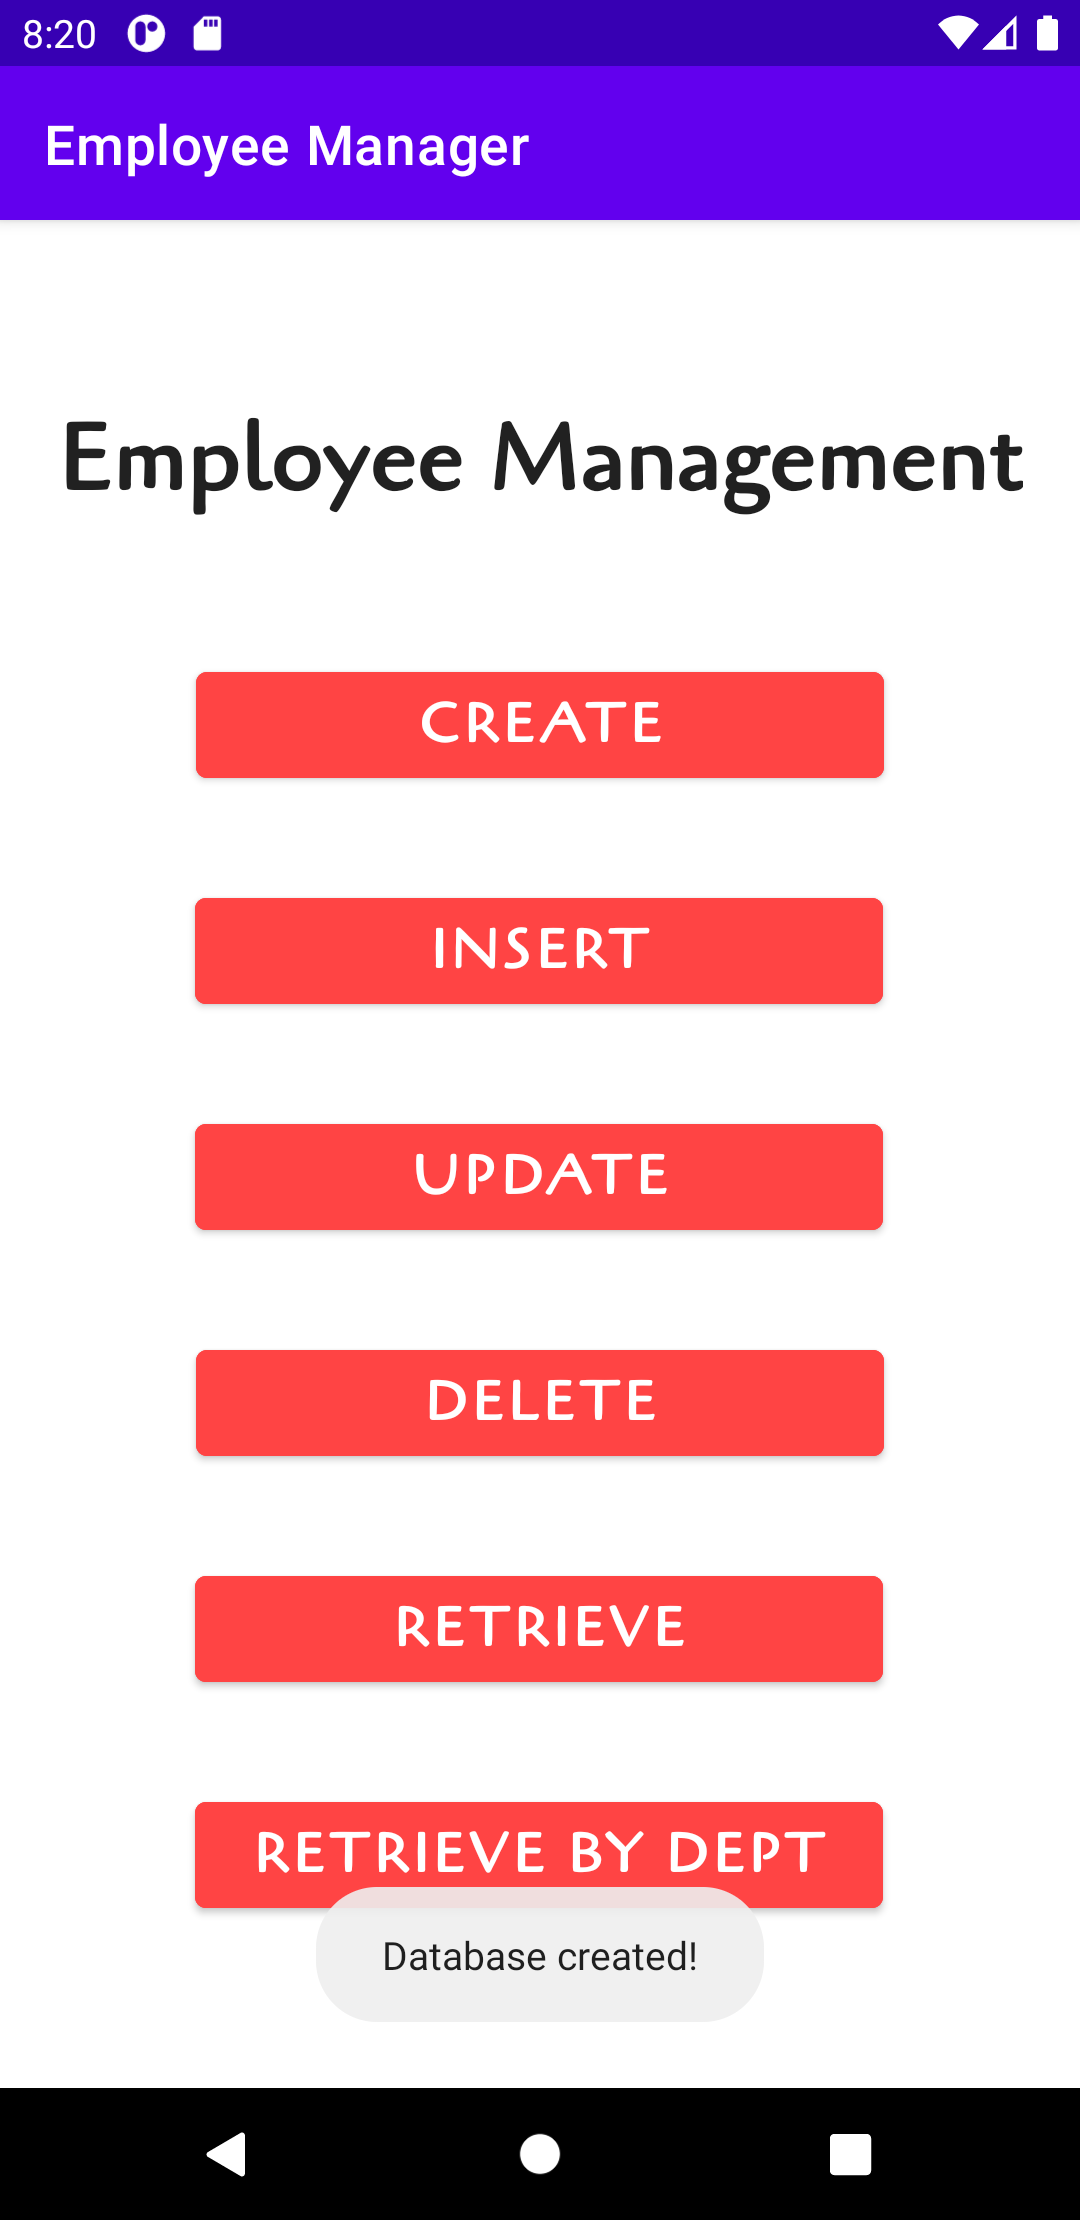
\includegraphics[height=15cm, width=7.3cm]{EmployeeManager/Screenshots/Output-1.png}
\end{figure}

%Output
\newpage
\subsection*{\flushleft{Output: Employee Manager - Insert Record:}}
\begin{figure}[h]
\centering
\caption{Output: Employee Manager - Insert Record.}
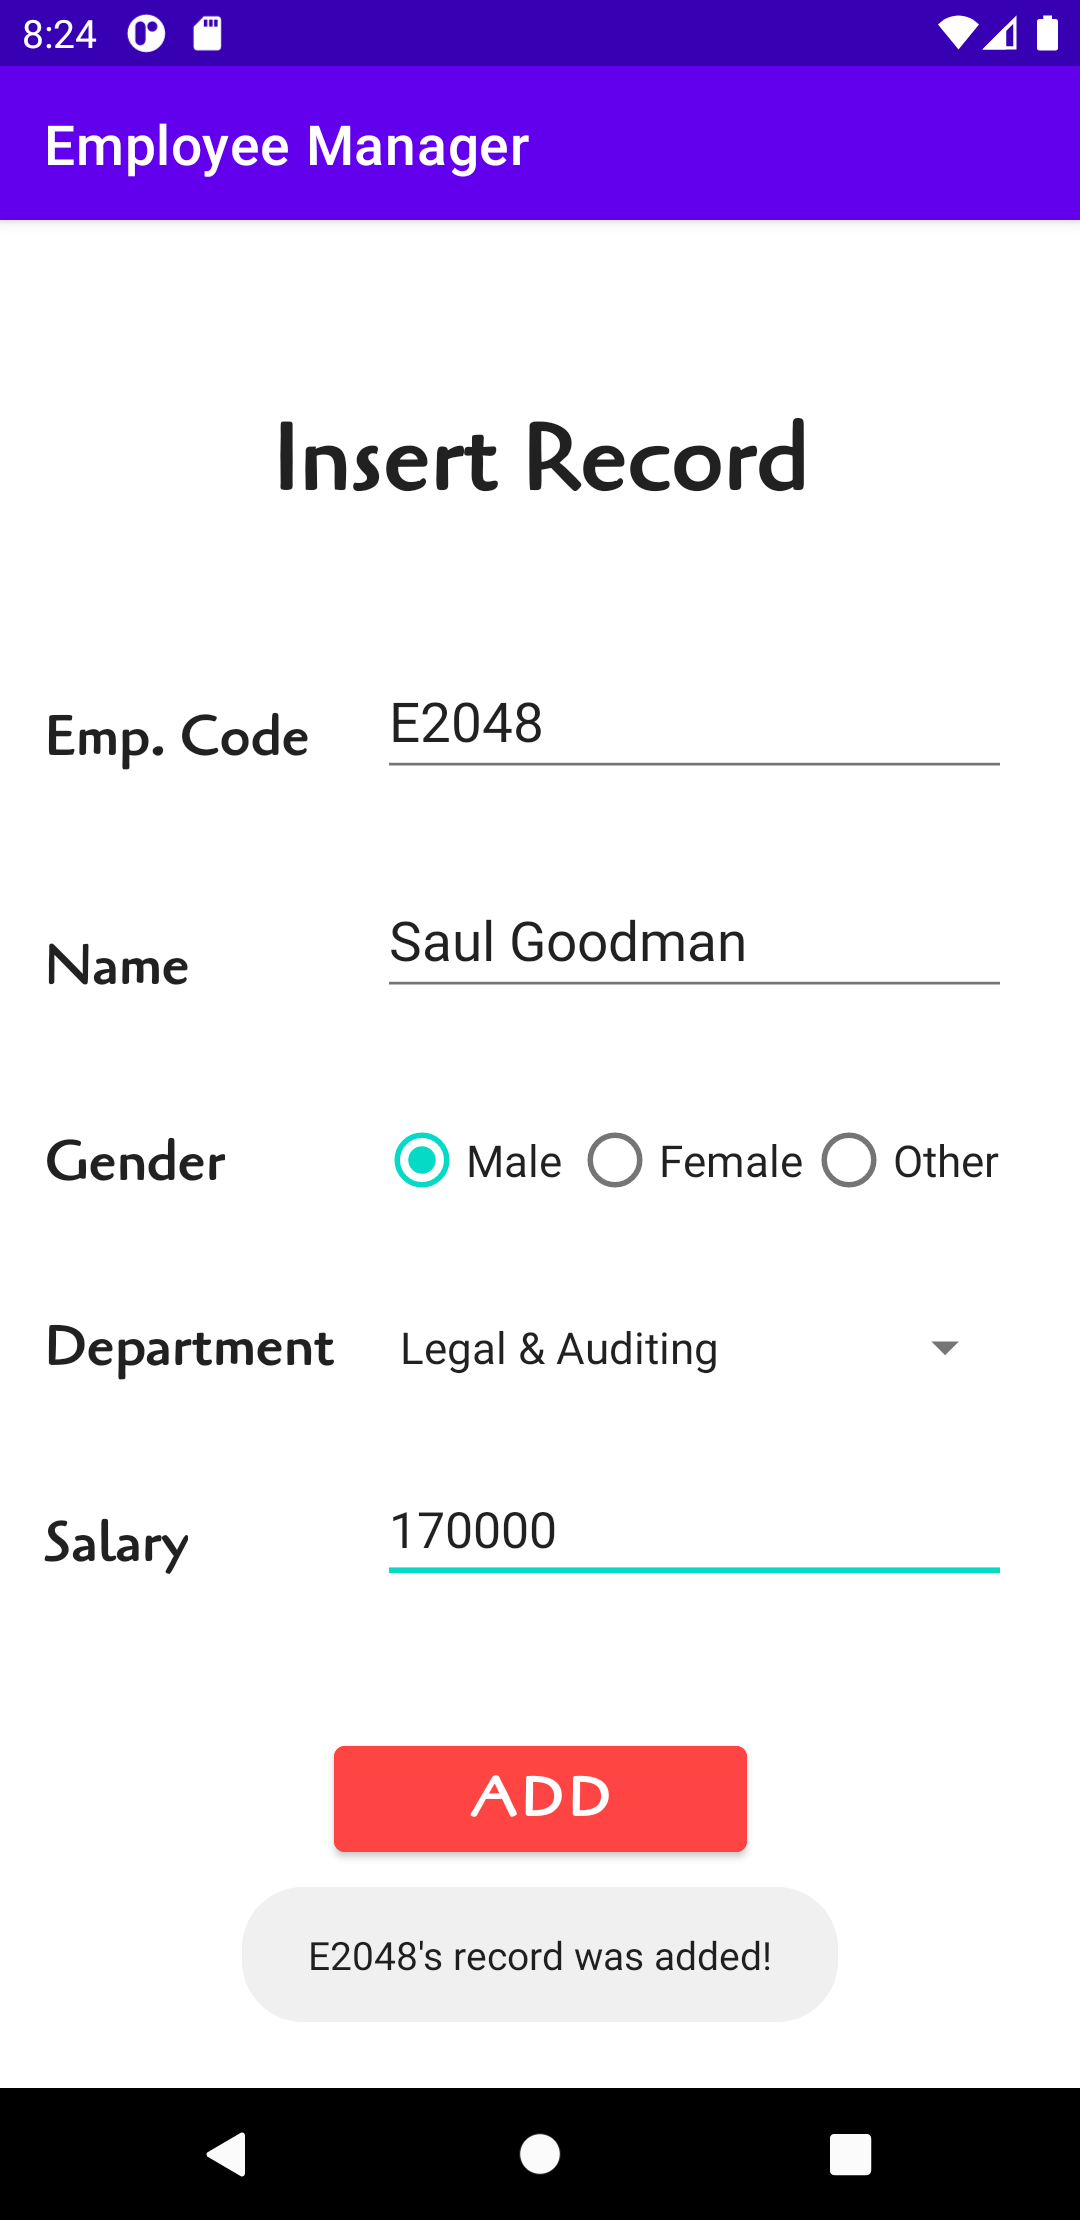
\includegraphics[height=15cm, width=7.3cm]{EmployeeManager/Screenshots/Output-2.png}
\end{figure}

%Output
\newpage
\subsection*{\flushleft{Output: Employee Manager - Retrieve Record:}}
\begin{figure}[h]
\centering
\caption{Output: Employee Manager - Retrieve Record.}
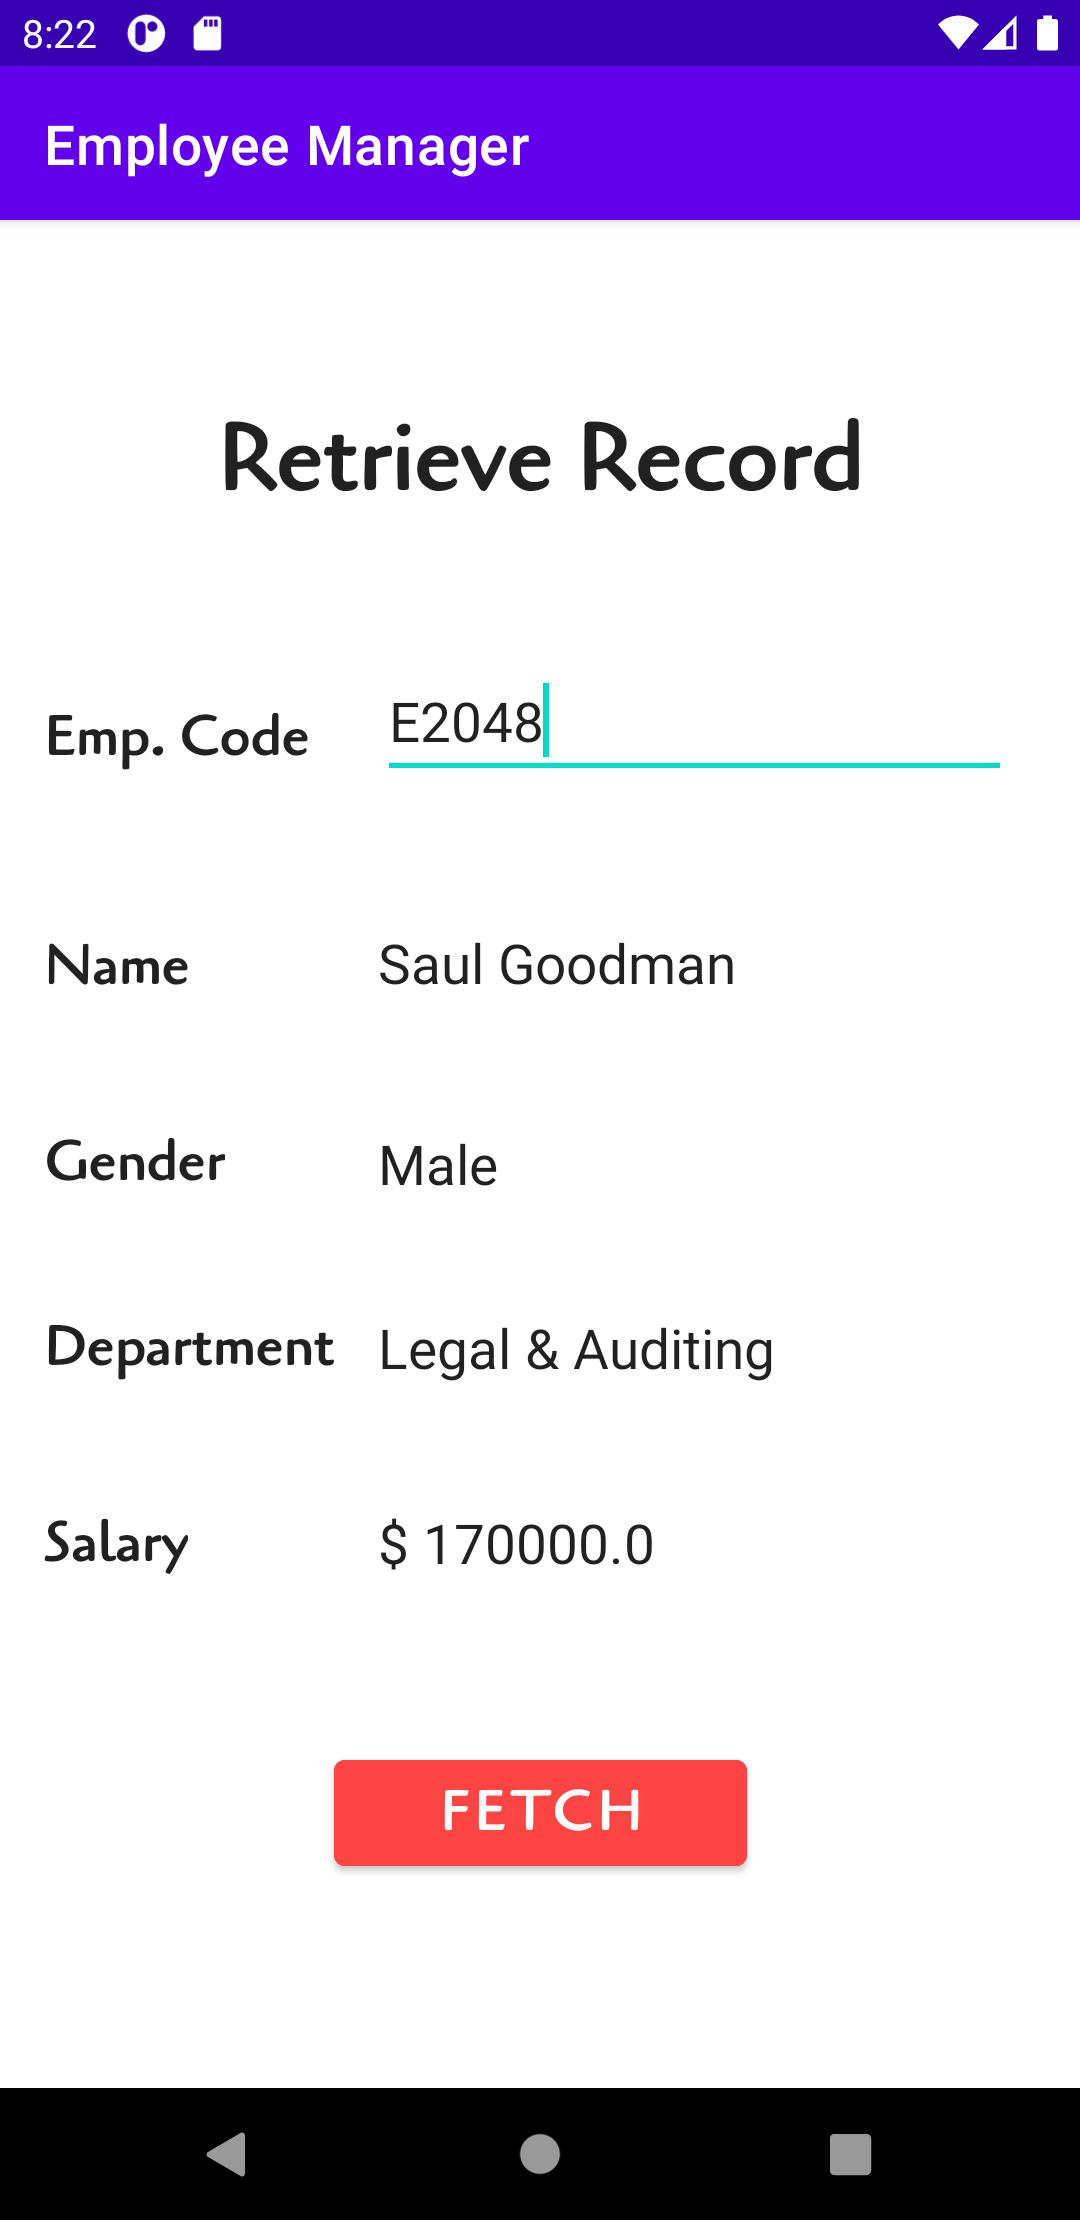
\includegraphics[height=15cm, width=7.3cm]{EmployeeManager/Screenshots/Output-3.png}
\end{figure}

%Output
\newpage
\subsection*{\flushleft{Output: Employee Manager - Update Record:}}
\begin{figure}[h]
\centering
\caption{Output: Employee Manager - Update Record.}
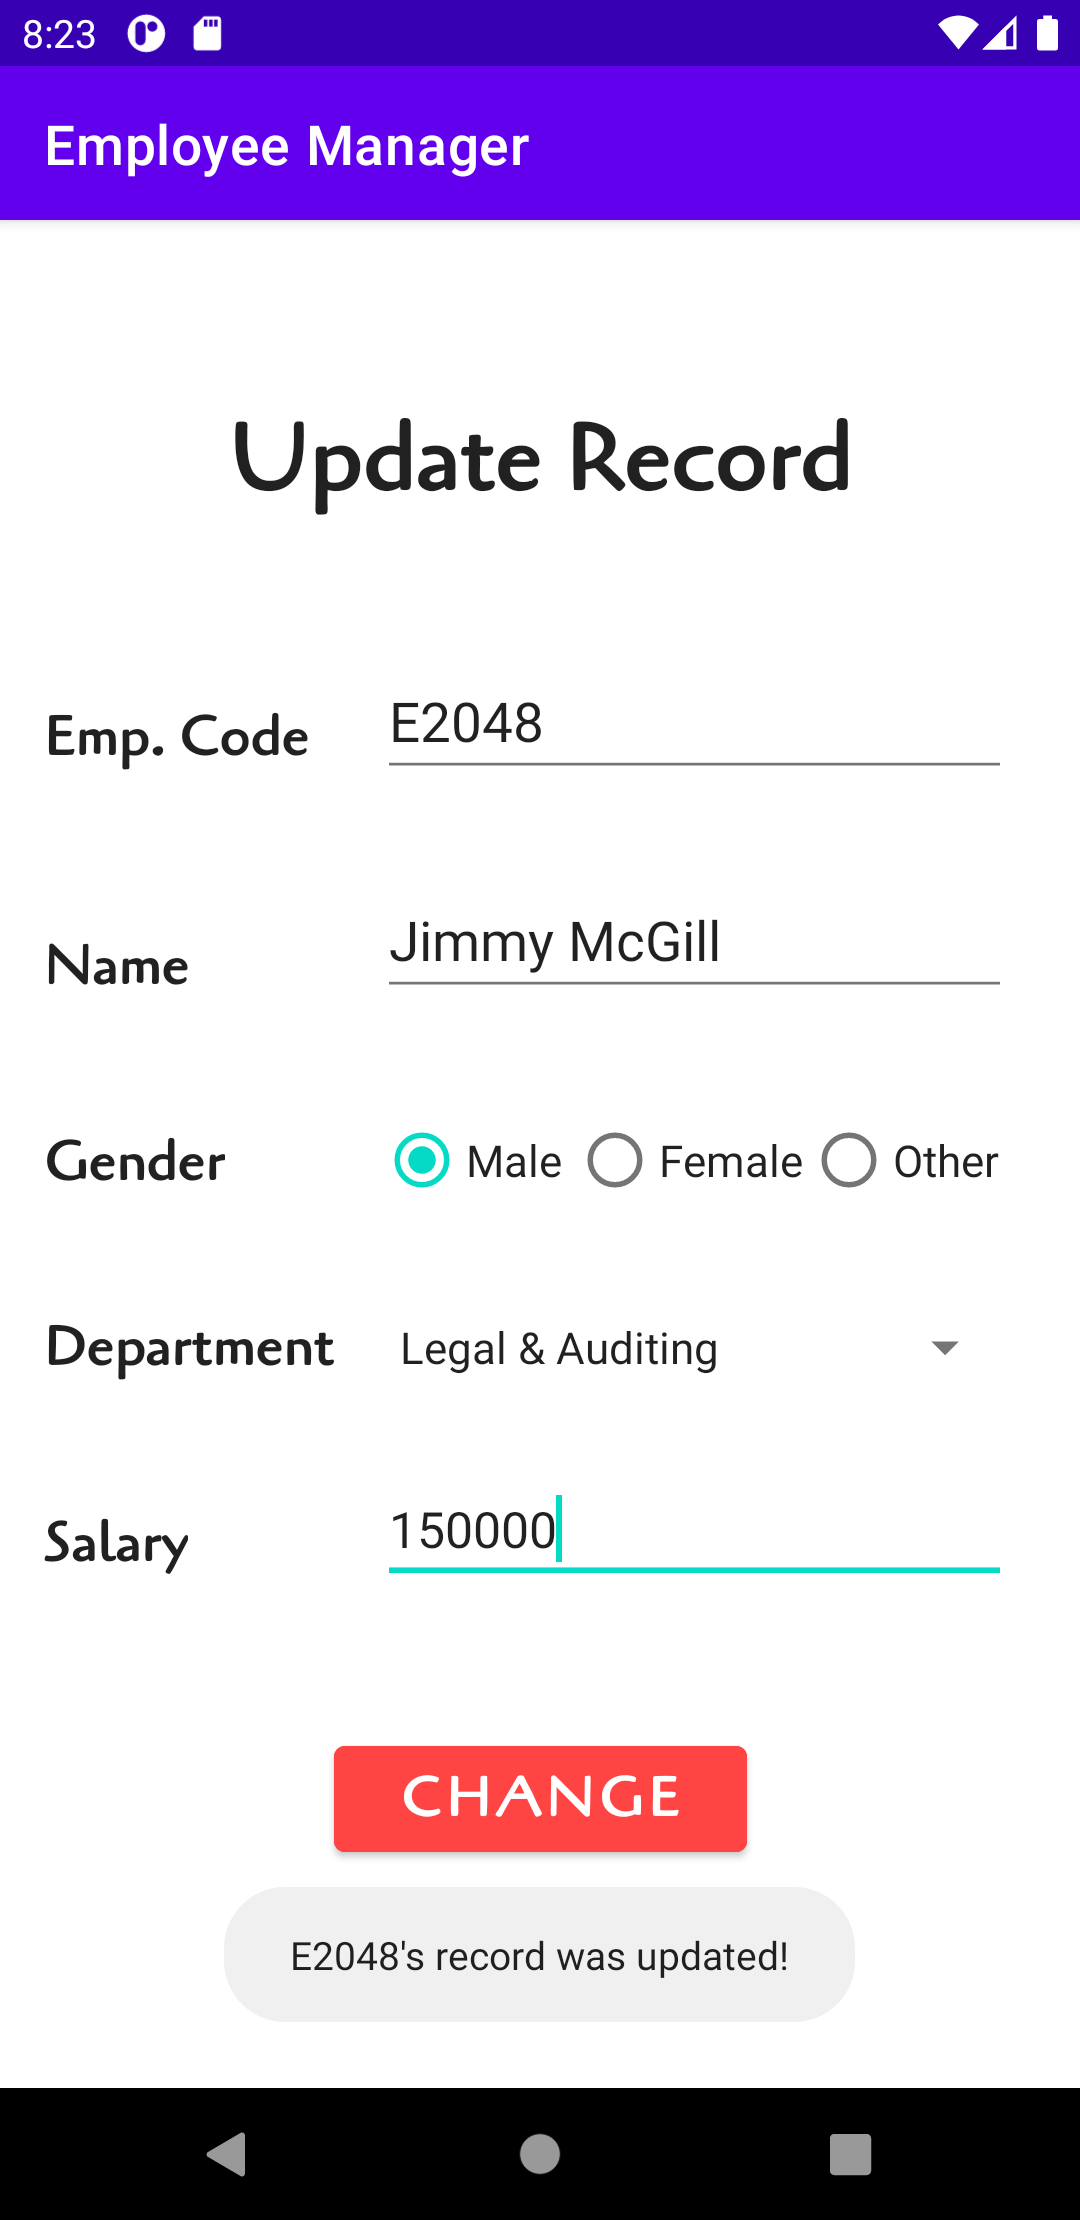
\includegraphics[height=15cm, width=7.3cm]{EmployeeManager/Screenshots/Output-4.png}
\end{figure}

%Output
\newpage
\subsection*{\flushleft{Output: Employee Manager - Retrieve Record:}}
\begin{figure}[h]
\centering
\caption{Output: Employee Manager - Retrieve Record.}
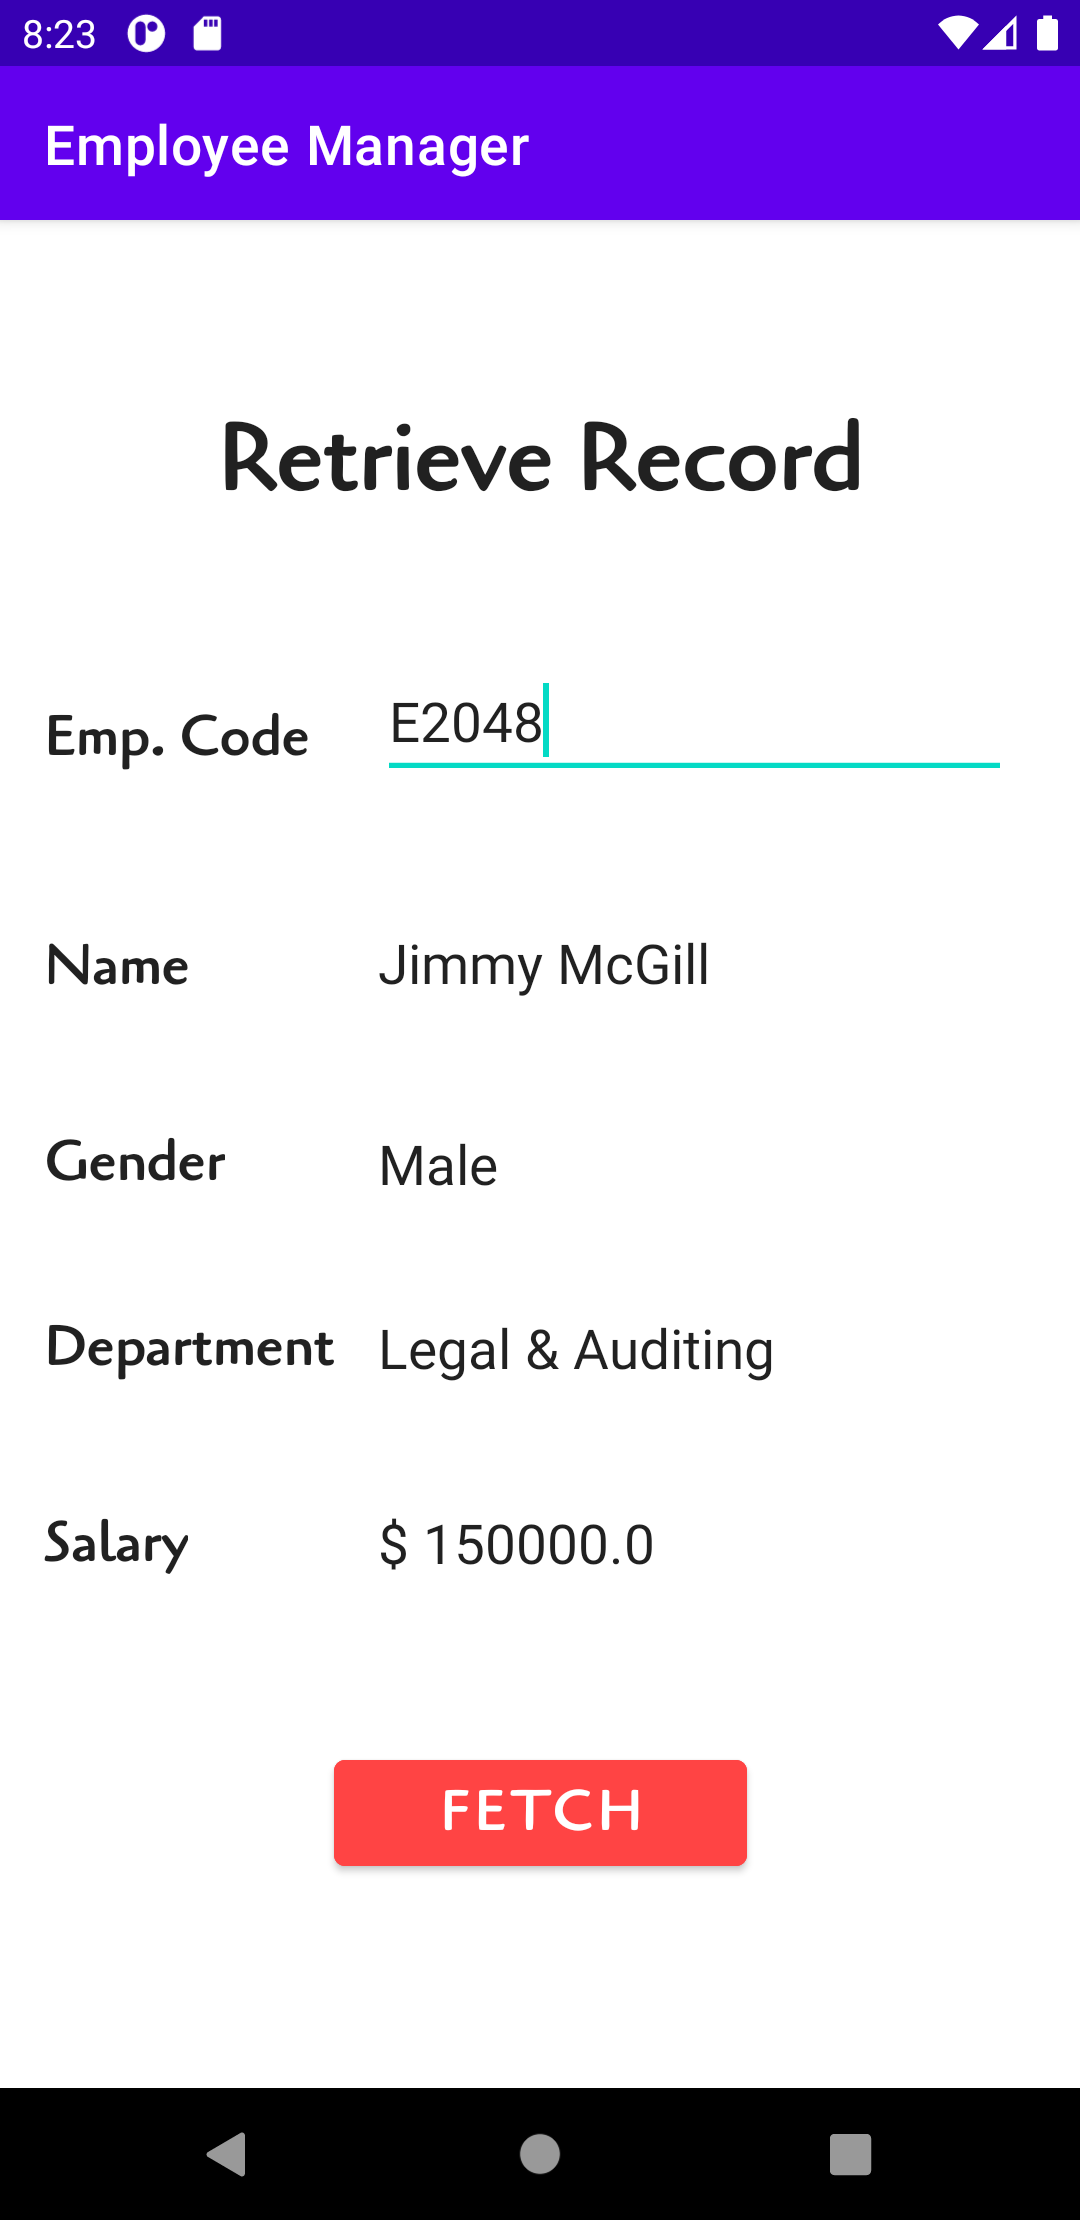
\includegraphics[height=15cm, width=7.3cm]{EmployeeManager/Screenshots/Output-5.png}
\end{figure}

%Output
\newpage
\subsection*{\flushleft{Output: Employee Manager - Delete Record:}}
\begin{figure}[h]
\centering
\caption{Output: Employee Manager - Delete Record.}
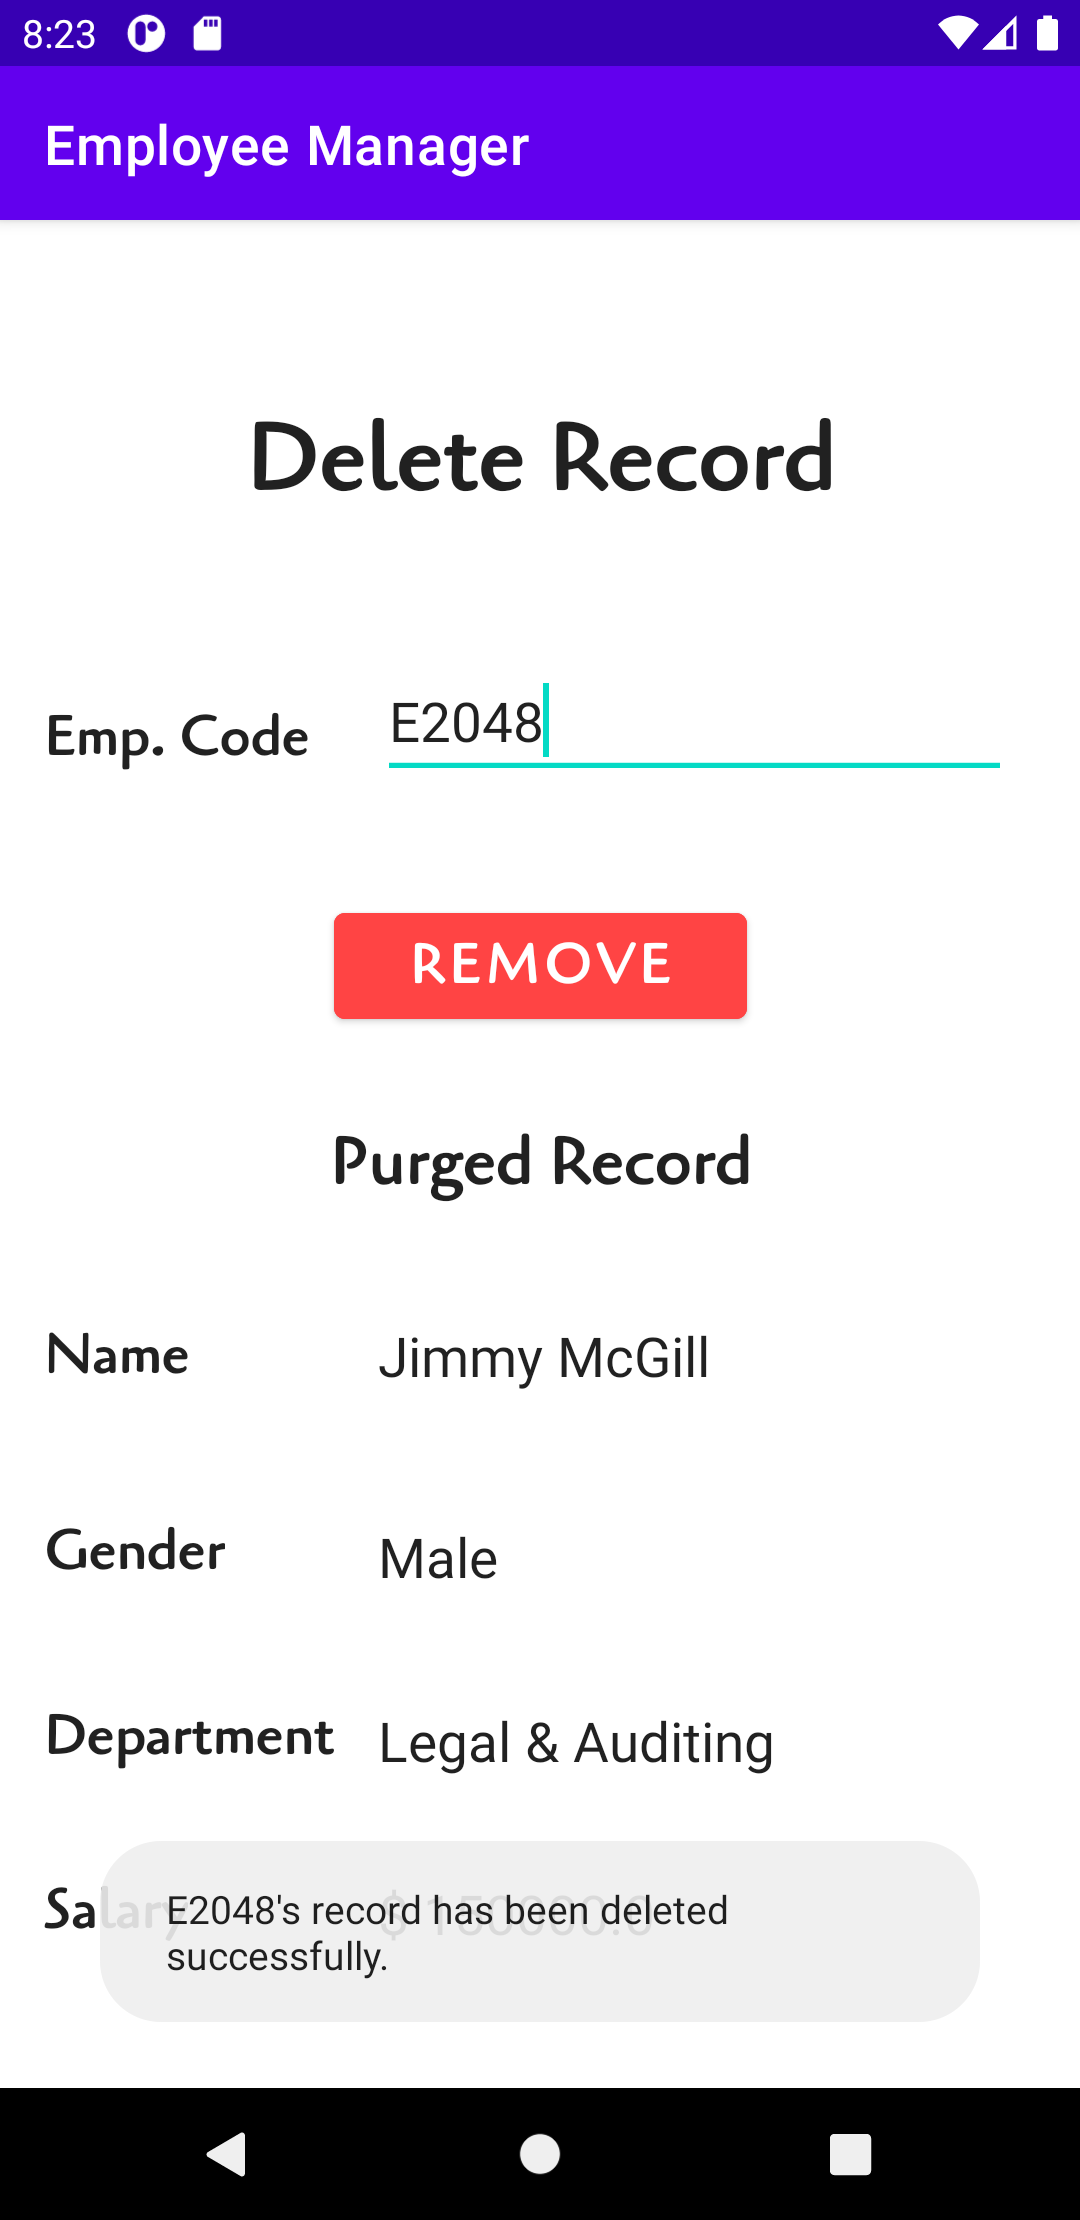
\includegraphics[height=15cm, width=7.3cm]{EmployeeManager/Screenshots/Output-6.png}
\end{figure}

%Output
\newpage
\subsection*{\flushleft{Output: Employee Manager - Retrieve Records By Department (1):}}
\begin{figure}[h]
\centering
\caption{Output: Employee Manager - Retrieve Records By Department (1).}
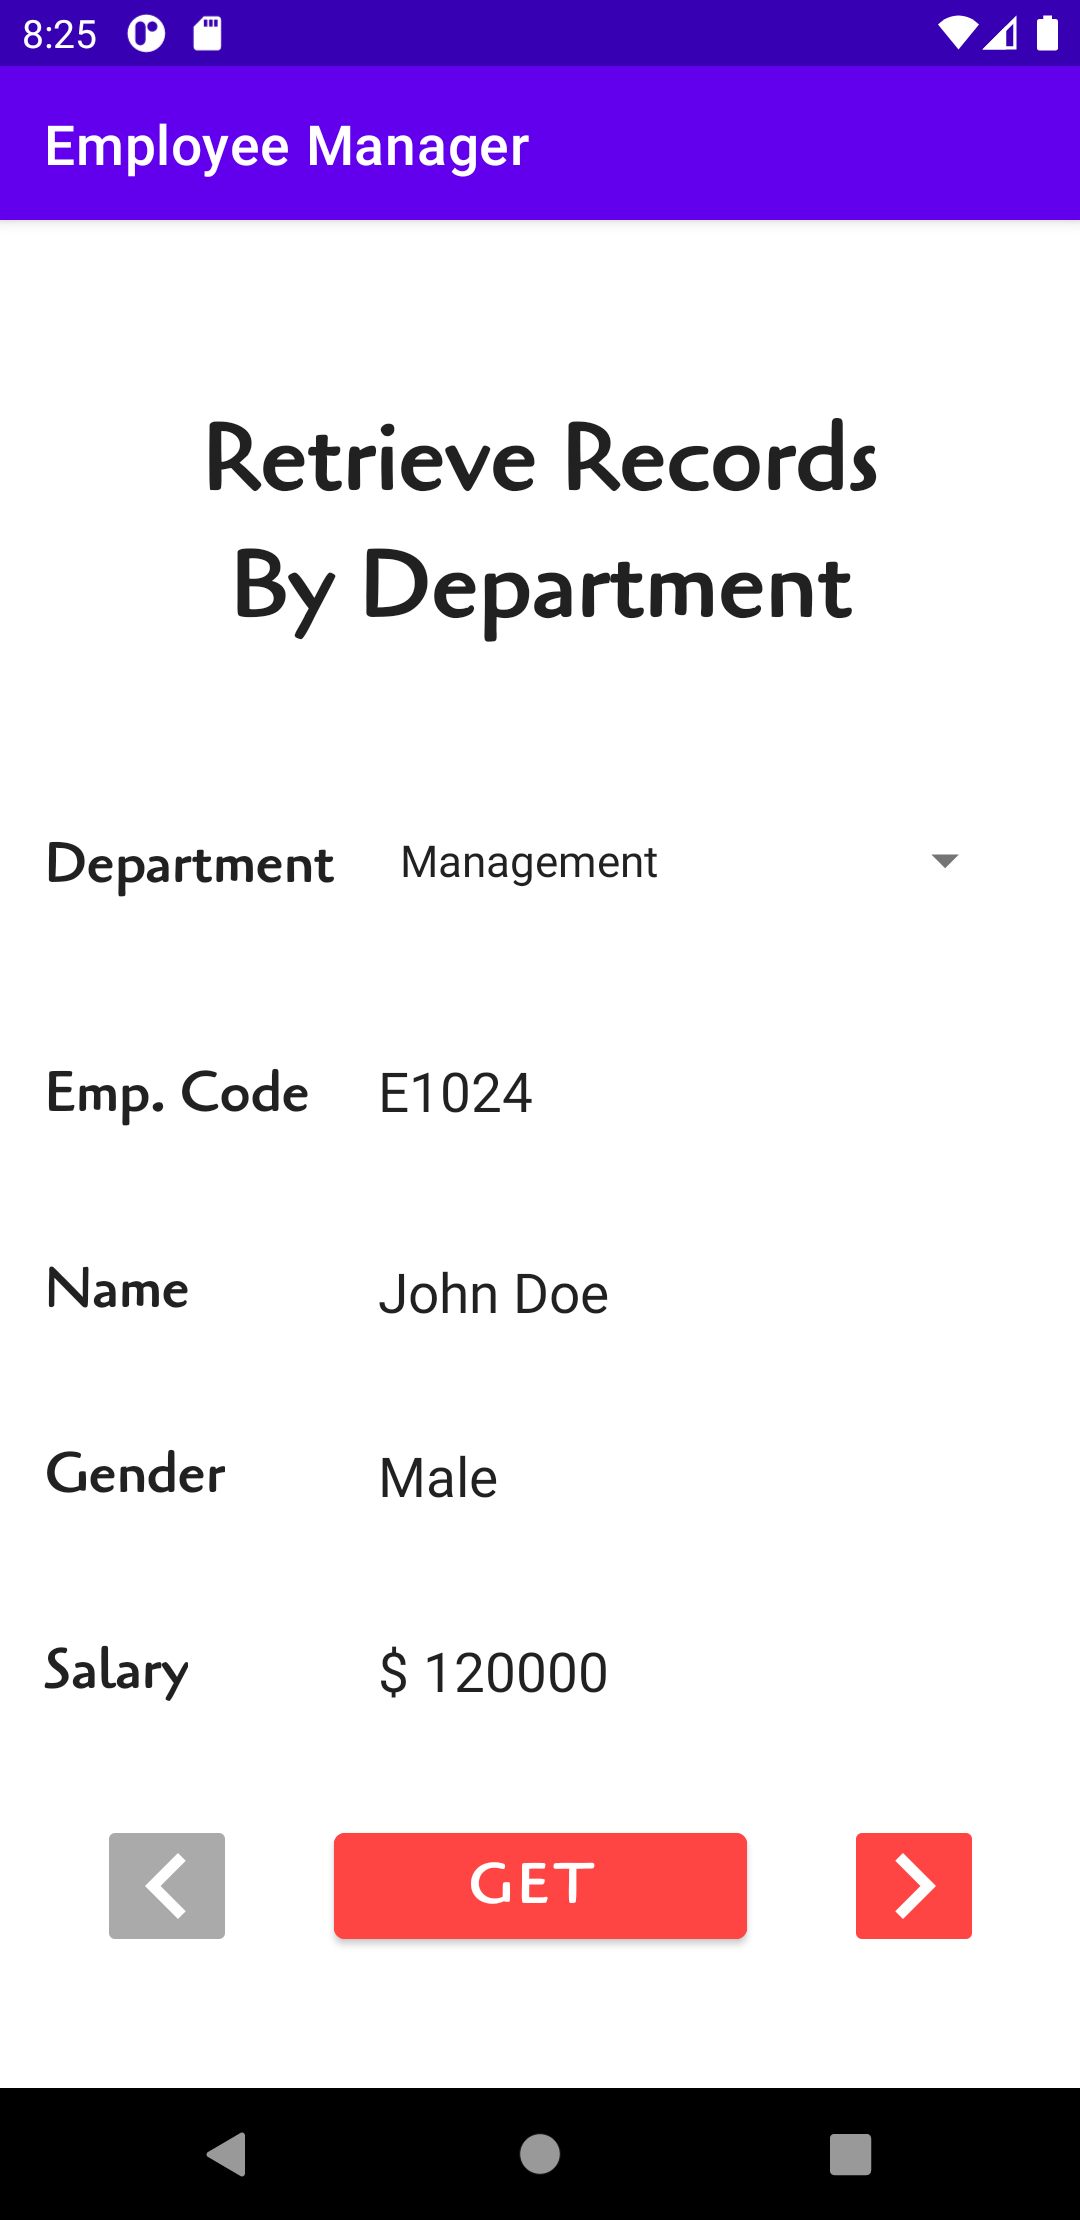
\includegraphics[height=15cm, width=7.3cm]{EmployeeManager/Screenshots/Output-7.png}
\end{figure}

%Output
\newpage
\subsection*{\flushleft{Output: Employee Manager - Retrieve Records By Department (2):}}
\begin{figure}[h]
\centering
\caption{Output: Employee Manager - Retrieve Records By Department (2).}
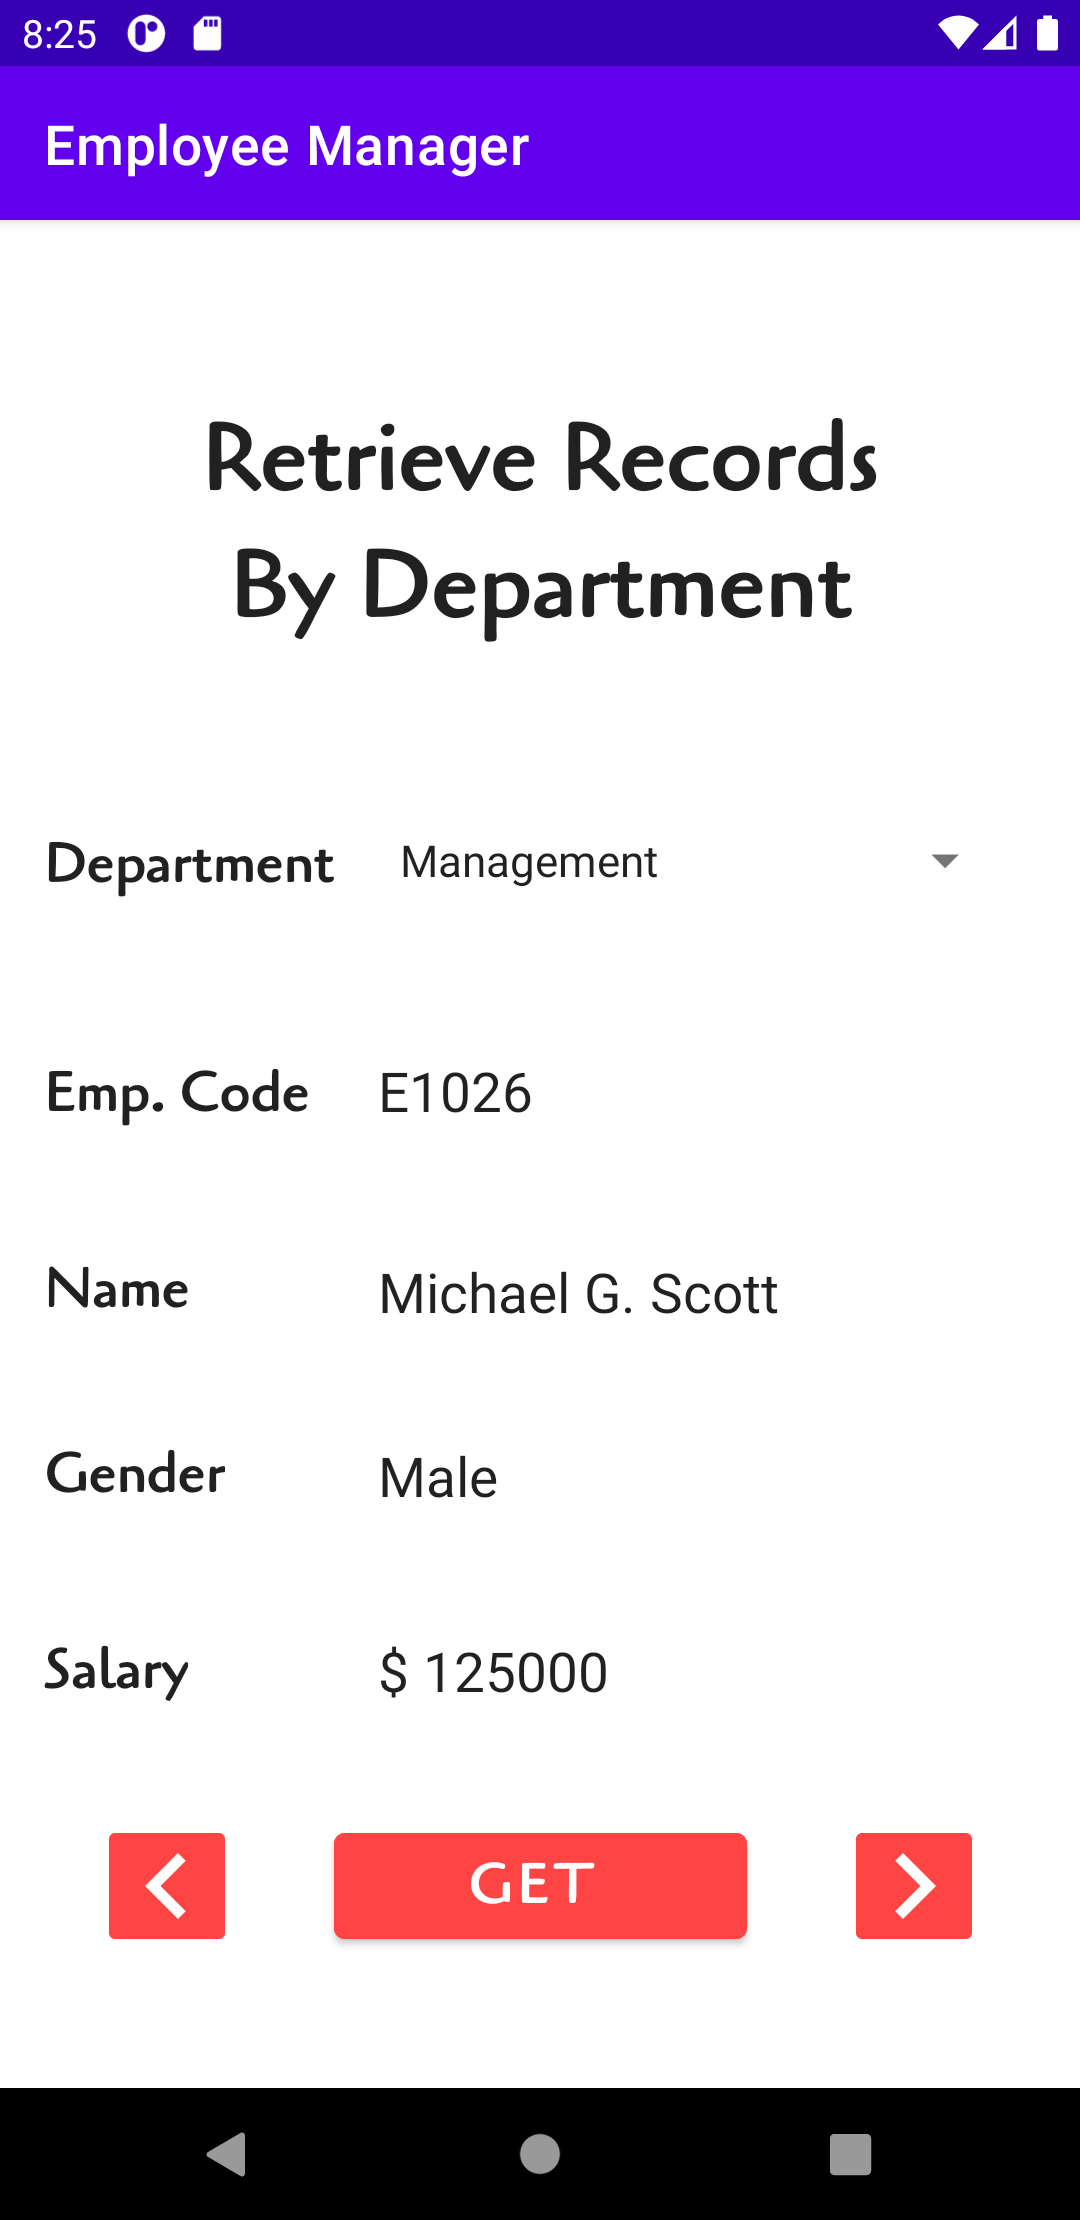
\includegraphics[height=15cm, width=7.3cm]{EmployeeManager/Screenshots/Output-8.png}
\end{figure}


%Learning Outcome
\newpage
\subsection*{\flushleft{Learning Outcome:}}
\begin{itemize}
\item I understood Android makes use of \textbf{SQLite} for its database purposes, and why SQLite is preferred over a full-fledged DBMS service.
\item I learnt to implement a \textbf{Helper Class} extending from the \textbf{SQLiteOpenHelper Class} to construct methods for my own database handling.
\item I learnt about \textbf{SQLite Primitives} like \textbf{TEXT, NUMERIC, REAL, INTEGER, BLOB \& NULL}.
\item I implemented the mandatory \textbf{onCreate() and onUpdate()} methods in my helper class.
\item I was able to execute SQL Queries for \textbf{Creating the Table, Inserting a Record, Updating a Record, Deleting a Record, Retrieving Records by Emp. Code \& Retrieving by Department} in the helper class and provided a facade to access the query results for the main program.
\item I learnt how to traverse \textbf{Cursor} objects that are returned by SQLite methods on execution of a SELECT query.
\item I learnt how to alert users with the help of small \textbf{Toast} messages in Android.
\item I was able to implement the CRUD operations along with the Retrieve By Department operation as dictated by the objective of the program.
\item I learnt to use \textbf{TextUtils} for validating user-input and \textbf{RegEx} to check for numbers in a given string.
\item I was able to design a \textbf{navigator} using \textbf{$<$ \& $>$ buttons} to traverse through multiple records returned from the Retrieve by Department query.
\item I learnt how to change \textbf{BackgroundTint} for buttons programatically, to highlight enabled/disabled behaviour.
\item I learnt basics of \textbf{SQLite Programming in Android}.

\end{itemize}


\end{document}